\documentclass[landscape,final,a0paper,10pt]{baposter}

\usepackage{graphicx}
\usepackage{url}
\usepackage{multicol}
\usepackage{enumitem}
\usepackage{bm}
\usepackage{relsize}
\usepackage{multirow}
\usepackage{rotating}

%\setlength{\columnsep}{1.5em}
%\setlength{\columnseprule}{0mm}

\graphicspath{{./images/}{../images/}}


\definecolor{darkblue}{HTML}{0000FF}
\definecolor{lightblue}{HTML}{00AAAA}
\definecolor{lightestblue}{HTML}{00FFFF}

\hyphenation{resolution occlusions}

\newcommand{\compresslist}{%
\setlength{\itemsep}{1pt}%
\setlength{\parskip}{0pt}%  
\setlength{\parsep}{0pt}%
}

\begin{document}

\begin{poster}
{
	grid = false,
	columns=3,
	bgColorOne = lightestblue,
	borderColor = lightblue,
	headerColorOne = white,
	headerFontColor = black,
	boxColorOne = white,
	textborder = rounded,
	eyecatcher = true,
	headerborder = closed,
	headerheight = 0.1\textheight,
	headershape = smallrounded,
	headershade = plain,
	headerfont =  \Large\bf\textsc,
	textfont = {\setlength{\parindent}{1.5em}},
	boxshade = plain,
	background = plain,
	linewidth = 2pt
}
{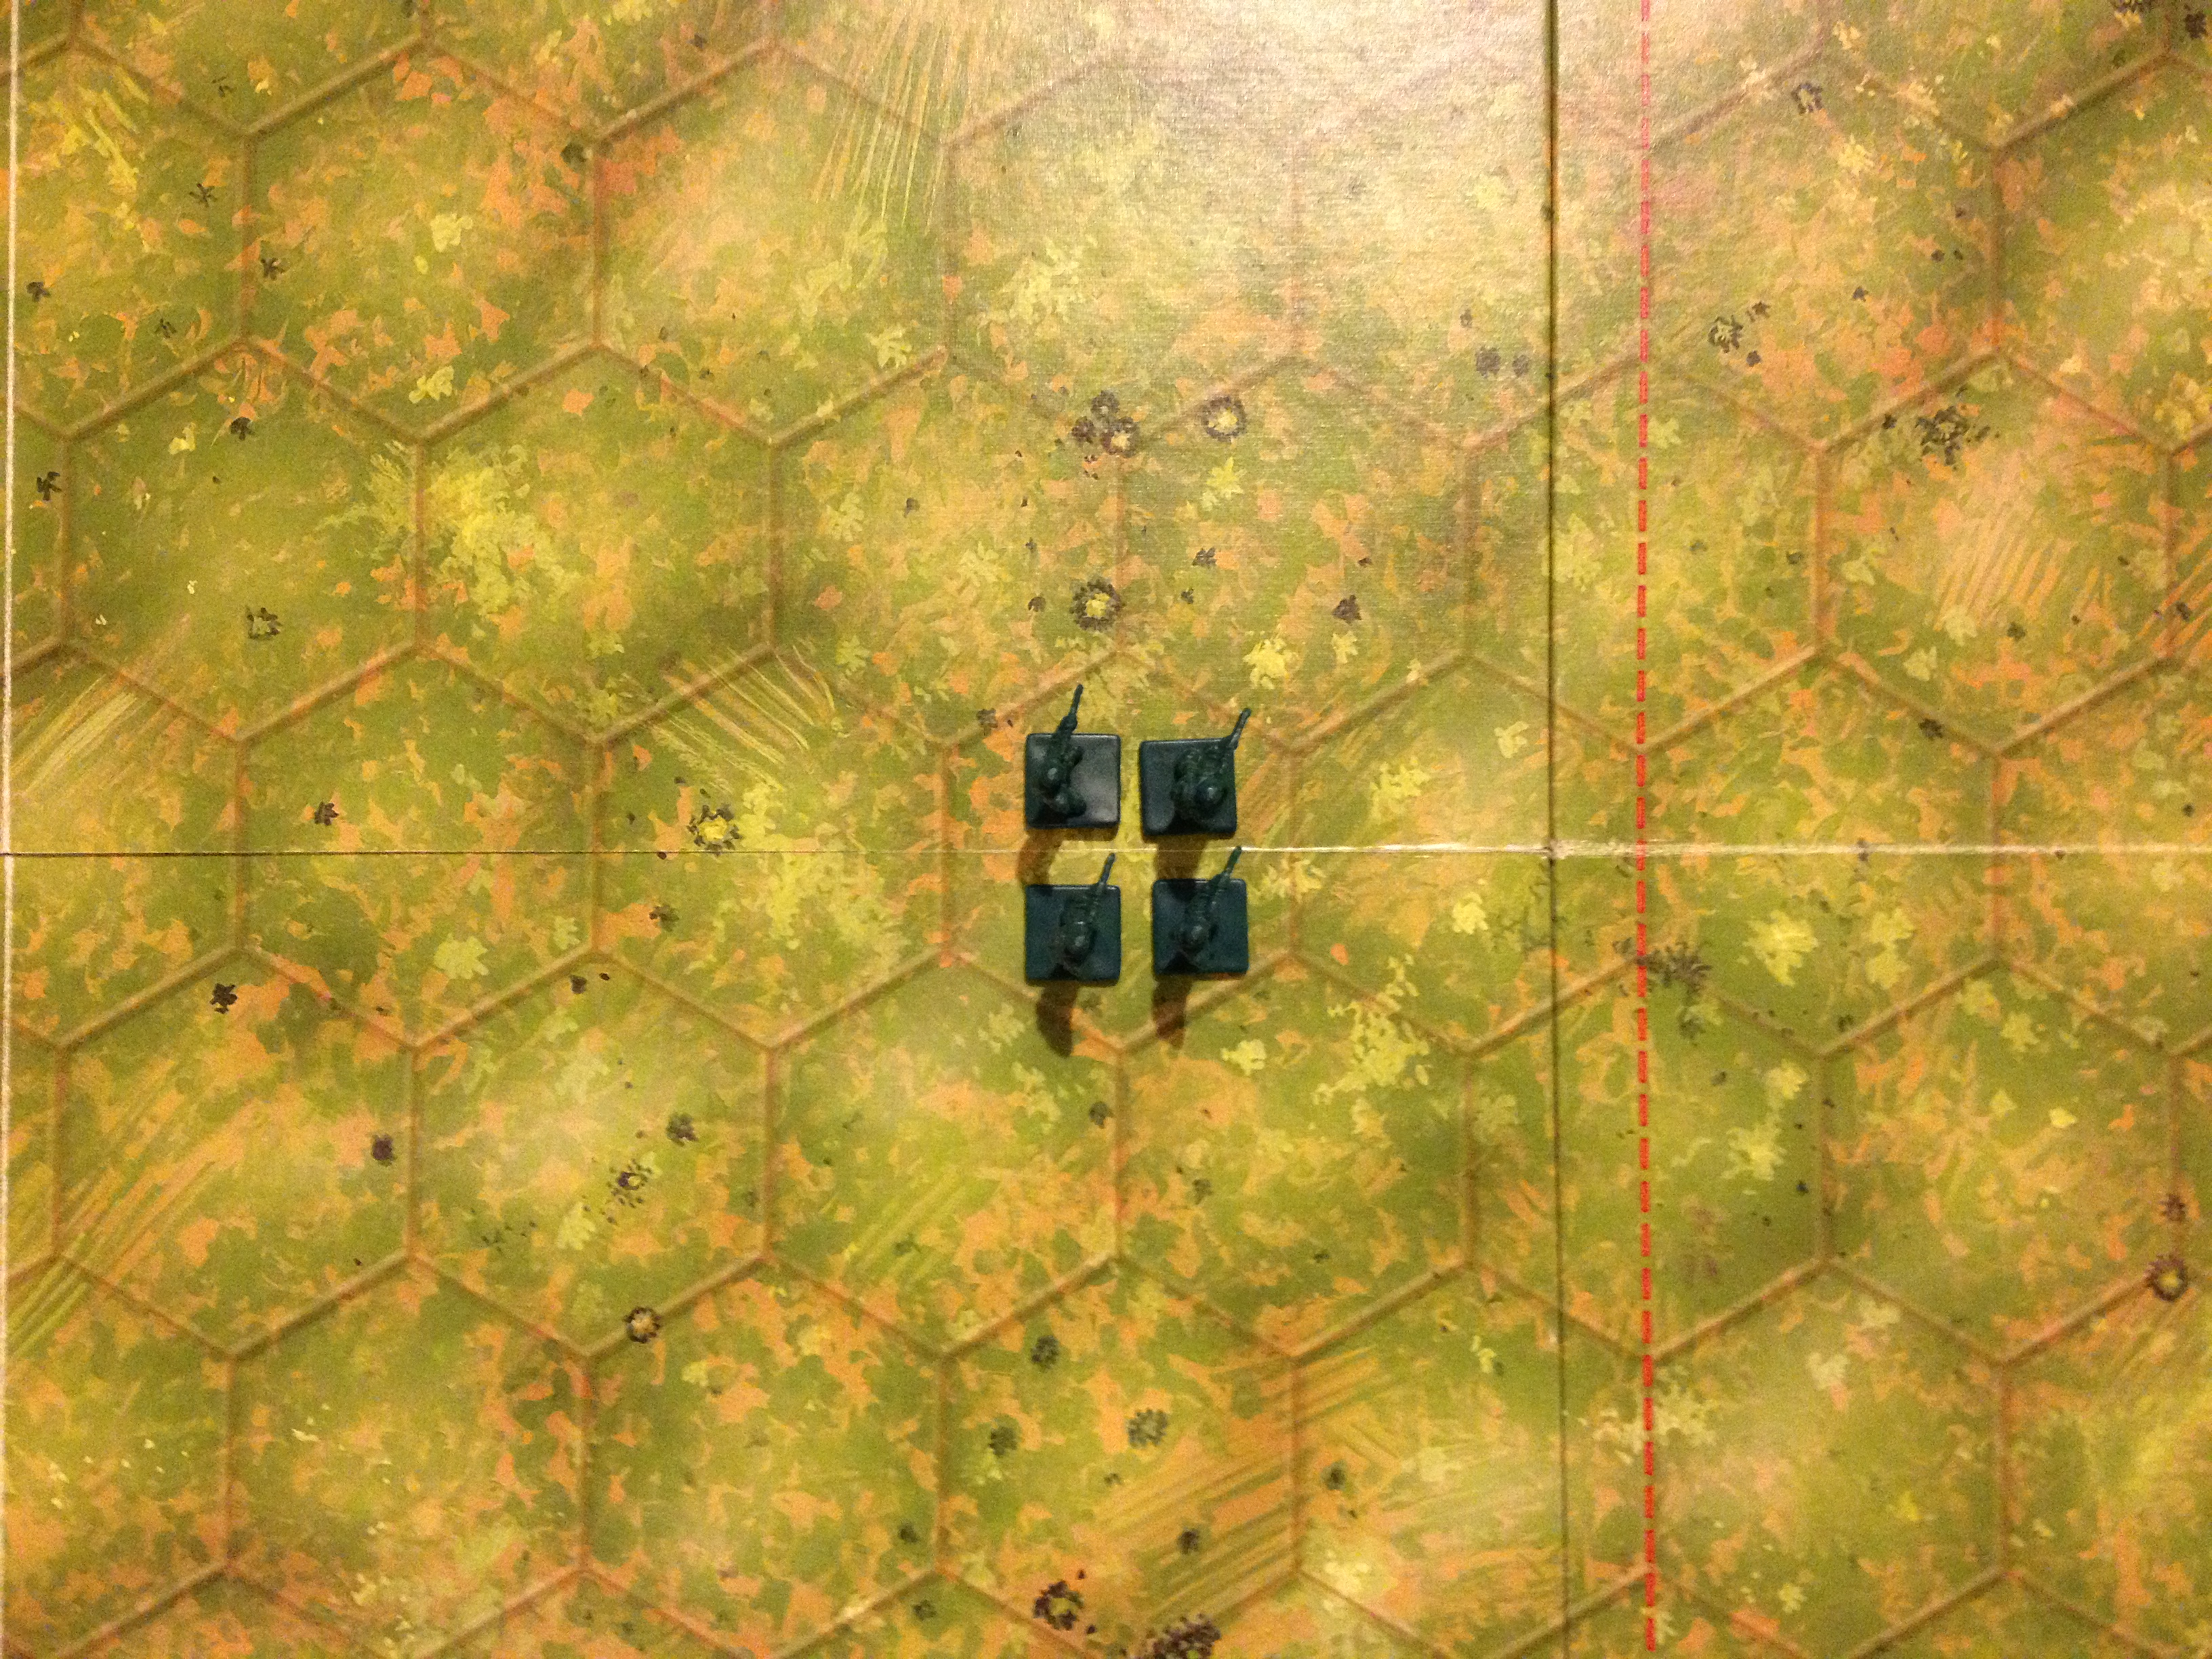
\includegraphics[height=6em]{../images/board_1}}
{\bf\textsc{Desert Fox: a Simple Wargame AI}\vspace{0.5em}}
{\textsc{Parker Michaelson}}
{
\includegraphics[height=6em]{../images/logo}}

\headerbox{Introduction}{name=intro, column=0, row=0}
{
Playing wargames, ranging from classics like Chess to Go to modern consumer games like Total War, presents a historically interesting problem for AI researchers.
Much progress has been made on the front of playing Chess and similar games with small search spaces and simple heuristics by using traditional search techniques.
Games with large search spaces which lack good heuristics, like Go, however, have presented a major challenge for such techniques.
Here we demonstrate the method of the {\it Monte Carlo Tree Search} for playing a simple game derived from the commercial game Memoir '44 called Desert Fox which, like Go, possesses a large search space and lacks effective heuristics.
}

\headerbox{General Strategy}{name=strategy, below=intro}
{
Desert Fox possesses a large search space compared to other games due to its simple, unrestrictive rules and large playing field.
On any given turn, a player may issue up to three orders to friendly units.
Orders may be to move to an adjacent tile, to fight an enemy unit on an adjacent tile, or to do nothing.
Play consists of alternating turns between the ``red'' and ``blu'' players until one of the players kills three enemy units.
This player wins the game regardless of the other player's score.
The board on which play occurs is rectangular in shape and consists of hexagons.
The board may be of any size so long as its width and height are odd for reasons specific to the implementation.
Each player is assigned enough units to span the width of the board, these units are placed at either length of the board as can be seen below.

\vspace{0.3cm}

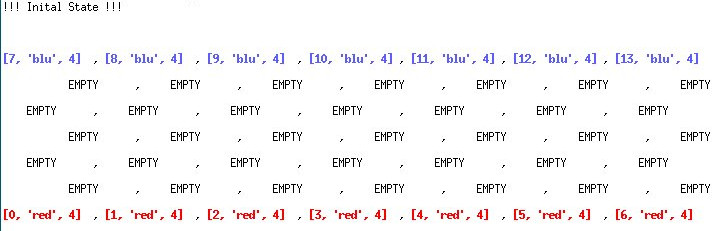
\includegraphics[width=0.9\colwidth]{../images/virtualboard_3.png}

\vspace{0.3cm}

The combination of many units and few restrictions leads to a swiftly growing combinatoric problem with an unreasonable size for a traditional unguided search.
Furthermore, a lack of good heuristics prevents both the implementation of a rule based player and the use of guided search techniques.
This project works around traditional limitations by using the Monte Carlo Tree Search (MCTS), which uses a large sampling of child states to find a close-to-optimal action for a given state.

%The MCTS algorithm is outlined below:

%\begin{enumerate}
%\item Generate a child state derived from the parent state by an action or series of actions. A heuristic may be used here, if available, to try and pick actions which generate close-to-optimal child states.
%\item Generate a terminal state from the child state by running a course of actions at random which are representative of a typical game.
%\item Evaluate the utility of the terminal state, and backtrack to the parent state while updating each child state on the way with the utility information.
%\item Repeat steps 1-3 until computational budget is exhausted.
%\item Pick the action which yields the ``best'' child.
%\end{enumerate}

%The ``best'' child depends on the situation the algorithm is being used in.
%It may be that the algorithm should value the average performance of a child node, or it may attempt to have a certain lower bound on performance, or one of any number of rules.
%The implementation of MCTS used in Desert Fox has picks the child with the greatest average utility, utility here being the ratio of kills by the player to the total number of kills.
}

\headerbox{Results}{name=results, column=1, row=0}
{
To test the strength of the MCTS algorithm, a series of experiments was performed in which the algorithm played against against a control player making moves entirely at random.
The experimental parameters varied in the experiments were the size of the board, ranging from 3x3 to 7x7, and the time budget allocated to computing a single order, ranging from 1 millisecond to 10 seconds.
Three hundred experiments were conducted at each data point.
The graph below plots the number of games from this sample won by the AI player at each point.

\vspace{0.3cm}

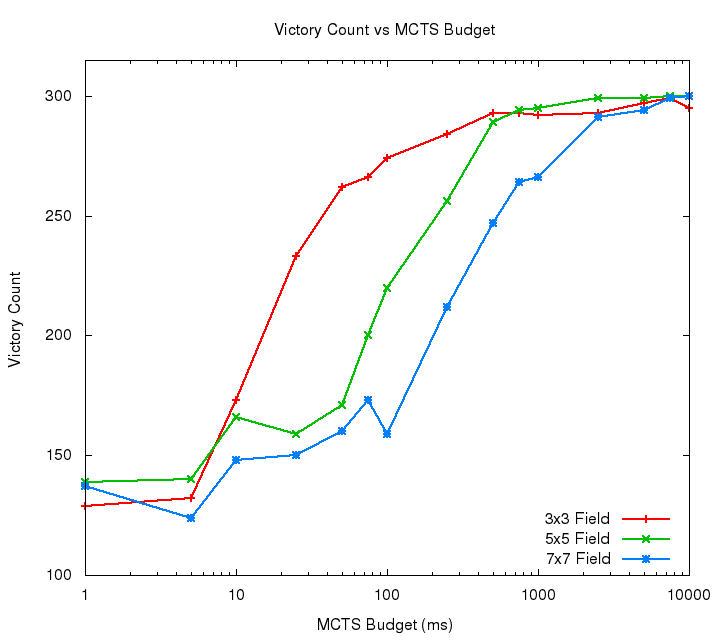
\includegraphics[width=0.9\colwidth]{../images/lineplot}

\vspace{0.3cm}

A strong correlation is noted between the budget afforded to the MCTS algorithm and the number of games won by the AI player.
The number of wins by the AI player increased to almost 100\% of the sample when 10 seconds were allocated per decision for all board sizes.
This effect is a direct result of the MCTS algorithm having more time to sample potential moves, improving its chances of finding a close-to-optimal move.

There also exists an inverse correlation between the size of the board played on and the win-rate for several budgets.
That is to say that the MCTS algorithm performed better on the smaller of any two boards for a given time budget.
%This is because the size of the search space grows exponentially with the size of the board.
This is because for small boards and the associated small search spaces, the sample of states taken by the MCTS algorithm can encompass a significant fraction of possible outcomes.
As the board gets larger the search space grows by an exponential amount, decreasing the size of the sample relative to the search space by an exponential factor as well.
This in turn leads to samples which are less representative of the search space, impeding the ability of the MCTS algorithm to make close-to-optimal decisions.
}

\headerbox{Results (cont.)}{name=cont, column=2, row=0}
{
As a final note on the results, a double tailed t-test was performed on all data points, the null hypothesis being that the AI player had performance equivalent to a control player, in which case the expected outcome of a match would be wins 50\% of the time for the AI player.
The results of the t-test indicated that all data points with time budgets greater than 500 milliseconds showed a statistically significant difference from the null hypothesis with confidence \(>95\%\).
This shows that for all time budgets greater than 500 milliseconds, the AI player performs better than a control player.
Interestingly, the inferior performance of the AI player relative to the control player on the 3x3 board for budgets less than 10 milliseconds and on the 7x7 board at 5 milliseconds is also statistically significant, indicating that the MCTS algorithm actually performs worse than random for extremely small time budgets.
The cause of this phenomenon is not known, and it may simply be a statistical aberration.
}

\headerbox{Conclusion}{name=conclusion, column=2, below=cont}
{
Based on the performance of MCTS algorithm in the experimental trials, we see that for large search spaces MCTS is a viable AI agent.
Furthermore, we see that the performance of MCTS improves in a roughly logarithmic manner with the increase of the computation budget.
%In smaller search spaces or with low computation budgets, the performance of MCTS tends to be equal to or worse than an algorithm picking moves at random while also being much slower than the random player.
%This logic extends to suggest that a rule-based AI system like a reflex agent may be able to outperform MCTS in similar conditions.

It is reasonable to speculate that promising future work in this area should focus on,

\begin{itemize}
\item increasing the strength of an MCTS algorithm by increasing the number of simulations that can be performed within the computational budget, or
\item by adding a learning system, such as Q-Learning, as a heuristic to better focus the attention of an MCTS algorithm on promising actions or to improve the prediction and computation of terminal states.
\end{itemize}

In either case, the future of the MCTS algorithm promises a significant advantage over traditional searches in large search spaces.
}

\headerbox{Useful Works}{name=references, column=2, below=conclusion}
{
\begingroup
% Fix ref issue.
\renewcommand{\section}[2]{}%
\begin{thebibliography}{}

%  \bibitem{amato10}
%  High-level Reinforcement Learning in Strategy Games. Christopher Amato and Guy Shanai. {\it Proc. of 9\textsuperscript{th} Int. Conf. on Autonomous Agents and Multiagent Systems (AAMAS 2010).}

  \bibitem{brown09}
  A Survey of Mente Carlo Tree Search Methods. Browne, Powley, {\it et. al.}. {\it IEEE Transactions of Computational Intelligence and AI in Games, Vol. 4, No. 1, MARCH 2012.}

\end{thebibliography}
\endgroup
}

\headerbox{Source Code}{name=source, column=2, below=references}
{
The source code is available as a Git repository at:

\indent{    } \url{github.com/pcm2718/psychic-pikeman.git}
}

\end{poster}

\end{document}
